\documentclass[fleqn]{article}
\oddsidemargin 0.0in
\textwidth 6.0in
\thispagestyle{empty}
\usepackage{import}
\usepackage{amsmath}
\usepackage{graphicx}
\usepackage{flexisym}
\usepackage{calligra}
\usepackage{amssymb}
\usepackage{bigints} 
\usepackage[english]{babel}
\usepackage[utf8x]{inputenc}
\usepackage{float}
\usepackage[colorinlistoftodos]{todonotes}


\DeclareMathAlphabet{\mathcalligra}{T1}{calligra}{m}{n}
\DeclareFontShape{T1}{calligra}{m}{n}{<->s*[2.2]callig15}{}
\newcommand{\scriptr}{\mathcalligra{r}\,}
\newcommand{\boldscriptr}{\pmb{\mathcalligra{r}}\,}

\definecolor{hwColor}{HTML}{442020}

\begin{document}

  \begin{titlepage}

    \newcommand{\HRule}{\rule{\linewidth}{0.5mm}}

    \center

    \begin{center}
      
\includegraphics[height=11cm, width=11cm]{asu.png}
    \end{center}

    \vline

    \textsc{\LARGE Statistical/Thermal Physics}\\[1.5cm]

    \HRule \\[0.5cm]
    { \huge \bfseries Quiz 6}\\[0.4cm] 
    \HRule \\[1.0cm]

    \textbf{Behnam Amiri}

    \bigbreak

    \textbf{Prof: Michael Treacy}

    \bigbreak

    \textbf{{\large \today}\\[2cm]}

    \vfill

  \end{titlepage}

  By signing my name, I am promising that I did this quiz on my own without any outside help.

  \vspace{0.5cm}

  Name: \textbf{Behnam Amiri}

  \vspace{1cm}

  \begin{enumerate}
    \item A mass $m_1$ of water at temperature $T_1$ is mixed with a mass $m_2$ of water at temperature $T_2$
    in an insulated container whose heat capacity can be ignored. The specific heat of water is $C$.

    \begin{enumerate}
      \item Obtain an expression for the total entropy change that is generated by the mixing.

        % \textcolor{hwColor}{
        %   \\
        % }

    \end{enumerate}

    \item You are given the entropy function
    $$
      S(U, V)=a ~ ln \bigg( \dfrac{bV}{U^2} \bigg).
    $$
    $U$ is internal energy, $V$ is volume and $a, b > 0$ are constants. Show that this function gives
    negative temperatures when $U > 0$, and that it violates the third law of thermodynamics.

      % \textcolor{hwColor}{
      %   \\
      % }

    \item A cube has its six faces colored differently. It is aligned with a set of cartesian axes so that
    one of its corners is at the the origin, and three of its edges are on the $x, y, z$ axes.

    \begin{center}
      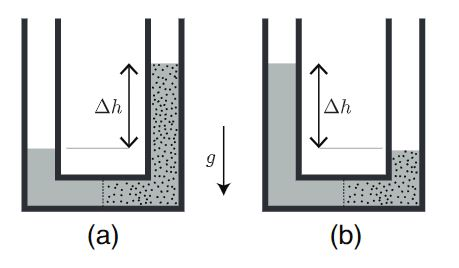
\includegraphics[height=5cm, width=6cm]{1.JPG}
    \end{center}

    \begin{enumerate}
      \item How many distinct orientations can the cube have?

        % \textcolor{hwColor}{
        %   \\
        % }

      \item 1 mole of such cubes are neatly stacked face-to-face into a large $3D$ cubic array, with each
      cube randomly aligned in one of its orientations. What is the entropy contribution arising
      from the orientational multiplicity of states?

        % \textcolor{hwColor}{
        %   \\
        % }

      \item What is the entropy contribution from orientations if the cube faces are all the same color?

        % \textcolor{hwColor}{
        %   \\
        % }

    \end{enumerate}

    \item Estimate the work done by the diatomic gas in the cycle $ABCD$ in the above $PV$ diagram.

    \begin{center}
      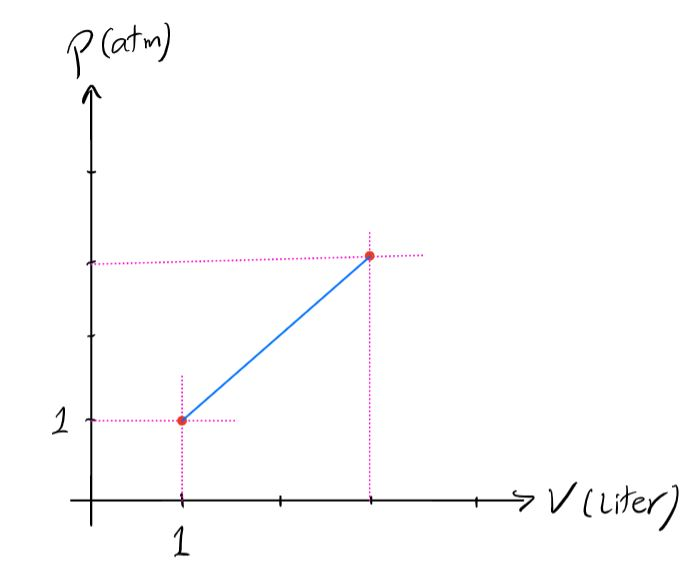
\includegraphics[height=8cm, width=10cm]{2.JPG}
    \end{center}

      % \textcolor{hwColor}{
      %   \\
      % }

  \end{enumerate}

\end{document}
